\chapter{Introduction}
\label{sec:intro}

\begin{figure}[t]
\centering
\includegraphics[width=\linewidth]{figures/qualitative_rotation.png}
\caption[Rotate-ID: One-shot personalized face rotation]{\textbf{Rotate-ID: One-shot personalized face rotation.} Given a \emph{single} reference image (left
column), methods spanning every personalization \emph{type}---adapter/encoder personalizers, the
per-identity fine-tuned DreamBooth, and instruction image-editors (Step1X-Edit, OmniGen2)---reproduce
the face but, bound by their frozen backbone's pose prior, degrade or refuse to rotate under large yaw
and profile views: the SD-adapter baselines stay near-frontal; DreamBooth, DreamO, and OmniGen2 turn
more but fall short of profile and drift off-identity; Step1X-Edit edits the face yet barely rotates.
Our \textbf{Rotate-ID} (right) re-poses the reference into arbitrary profile and
over-the-shoulder views while preserving identity. Each cell is annotated with its \emph{measured} head
yaw (green: turned; red: near-frontal); every Rotate-ID case shown matches \emph{both} the target yaw
and pitch, including the chin-down rows.}
\label{fig:teaser}
\end{figure}

Personalized text-to-image (T2I) generation, which renders a \emph{specific} human identity from one or a few reference photos, has become strikingly capable along nearly every axis except one: \emph{where the head is pointing}. Adapter-based methods inject a face embedding or identity tokens into a frozen diffusion backbone. IP-Adapter~\cite{ipadapter} uses decoupled cross-attention for an image prompt, PhotoMaker~\cite{photomaker} stacks ID embeddings, InstantID~\cite{instantid} couples a face encoder with an IdentityNet, and PuLID~\cite{pulid} and UniPortrait~\cite{uniportrait} further improve fidelity and multi-subject control. These methods can faithfully reproduce a face while varying style, attributes, and scene, but the head itself remains stubbornly near-frontal. This paper addresses \emph{posture-requested} personalization---the user's prompt names a target posture, and the system is accountable for realizing it---together with the \emph{pose-rectified} metrics needed to score such systems honestly.

\paragraph{What we mean by rotation.} We use a \emph{viewer-centric,
frame-referenced} convention (Fig.~\ref{fig:posedef}). A request to turn the head
``to the left'' means toward the \emph{left of the image frame} (the viewer's
left), not the subject's anatomical left; the head is \emph{turned left} or
\emph{turned right} once its yaw $\theta_y$ crosses $\pm15^\circ$, and \emph{chin
up} or \emph{chin down} once its pitch $\theta_p$ crosses $\pm15^\circ$
(Sec.~\ref{sec:metrics}). \emph{Over-the-shoulder} is an optional \emph{modifier}
on a turn, not a separate pose: it emphasizes the angle between head and chest, requiring the head to be turned far \emph{relative to the torso}
($|\Delta\theta_y|>25^\circ$), and places no constraint on where the body itself faces. These three rules---yaw, pitch, and the head-to-torso angle---are the
paper's complete pose vocabulary; every prompt is composed from them, and the
same rules score the generations (Sec.~\ref{sec:metrics}).

\begin{figure}[t]\centering
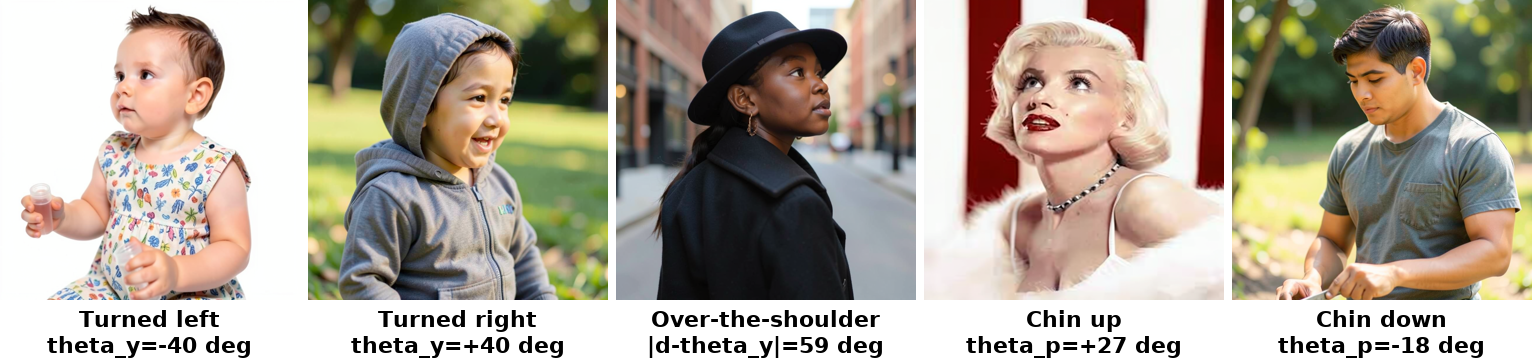
\includegraphics[width=\linewidth]{figures/pose_definitions.png}
\caption[Pose vocabulary]{\textbf{Pose vocabulary}, illustrated on \textbf{Rotate-ID} outputs and
annotated with the \emph{measured} angle that defines each category. \emph{Left/right}
turns are \emph{frame-referenced} (the viewer's, not the subject's), set by head yaw
$\theta_y$; \emph{over-the-shoulder} is a large head-to-torso angle
($|\Delta\theta_y|{>}25^\circ$), not merely a large head yaw; \emph{chin up/down} is
set by head pitch $\theta_p$. These are the pose dimensions our prompts control and
our metric verifies (Sec.~\ref{sec:metrics}).}
\label{fig:posedef}
\end{figure}

\paragraph{Why large turns fail: the pose--identity trade-off.}
Identity preservation and large-angle rotation are inherently in tension.
Large pose variation has long been recognized as a major challenge for face recognition and verification: profile faces are harder to match than frontal faces, and frontal-to-profile verification remains substantially more difficult than frontal-to-frontal matching~\cite{cfp, cao2018pose}.
A key reason is that face datasets and learned representations are often biased toward frontal or near-frontal faces; when the training distribution is biased in pose, recognition performance degrades on underrepresented extreme yaw cases~\cite{kortylewski2018empirical, cao2018pose}.
Thus, a single frontal reference provides increasingly weak identity constraints as the generated head turns toward large yaw, especially on the far side of the face where visible identity cues are reduced.

Existing personalizers can achieve high identity scores partly by avoiding this hard regime.
This behavior is consistent with prior observations in subject-driven and identity-preserving generation: identity-relevant information is often entangled with identity-irrelevant factors such as pose, background, expression, or other editable attributes, making it difficult to simultaneously preserve identity and satisfy strong control requirements~\cite{chen2023disenbooth, masterweaver, hu2025dynamicid, mishima2025facecrafter}.
Our experiments (Sec.~\ref{sec:exp}) show this pattern clearly: the strongest identity baselines keep most outputs near-frontal, so their high aggregate identity scores are measured mainly on easy frontal cases and drop sharply on the rare samples that actually reach large yaw.
We therefore evaluate identity \emph{at the pose actually produced}, rather than only reporting an aggregate score over all outputs (Sec.~\ref{sec:metrics}).


\paragraph{Why FLUX.2-klein?} We build on FLUX.2-klein, a distilled, few-step rectified-flow DiT---not a personalization model, and not trained with any identity-preservation objective. It is nonetheless viable as a one-shot identity substrate for two structural reasons. First, its VAE is a general-purpose, high-fidelity reconstruction codec: encoding and decoding a reference photo compresses it but does not discard identity-relevant visual detail. Second, its native in-context conditioning---the same mechanism it uses for structural and stylistic control~\cite{ominicontrol}---places a reference image's tokens in the same joint-attention sequence as the generation, where they are read directly by it. Neither property was designed for faces; together they mean a reference identity can survive generation without a dedicated ID-encoder branch, \emph{provided} the backbone's existing attention is directed to use it. We verify this causally in three steps---the VAE preserves identity-discriminative detail, and the joint attention (not token position alone) is what makes use of it, reading reference \emph{content} rather than merely occupying a sequence slot (Sec.~\ref{sec:refverify})---before showing that \emph{re-allocating} that attention is exactly what the identity levers below exploit (Sec.~\ref{sec:mechanism}). This is the premise Rotate-ID builds on, not an external face encoder grafted onto the backbone.

\paragraph{Approach.}
We present \textbf{Rotate-ID}, a one-shot personalization method built on a distilled few-step rectified-flow DiT (FLUX.2-klein) to address the pose--identity trade-off. Given a single identity image, Rotate-ID conditions \emph{in context} on structural pose control to drive explicit head rotation, including over-the-shoulder views. Because the structural control and the identity reference share one joint attention sequence, they inevitably compete for a single softmax-normalized attention budget---which is exactly where identity is lost under rotation. Rotate-ID reclaims that budget for identity in two steps. \emph{Reference duplication}---repeating the identity block to claim more of the shared budget---recovers most of the lost identity; and a \emph{learned attention-budget allocator} (the $\gamma$-gate), a $\sim$200-parameter, backbone-frozen module, generalizes this coarse, discrete heuristic into a continuous schedule over denoise steps and layers, \emph{refining} identity at the \emph{late} steps \emph{at no pose cost} and \emph{without editing the prompt}. Together---structural control for rotation, duplication and the gate for identity---these keep the head turning as instructed while the face stays stable.

\paragraph{Pose-rectified evaluation.} Progress on this task is also hard to \emph{read}: the dominant CLIP-based alignment score~\cite{clipscore} folds identity, pose, and scene into one opaque number (Sec.~\ref{sec:metrics} shows it cannot even say whether the requested head turn happened at all). We therefore propose a suite of \emph{pose-rectified performance metrics}. First, an \emph{explainable} pose check: a 3D estimator reads head and body orientation, their angles are mapped to discrete pose categories (left/right turn, over-the-shoulder, chin up/down), and we verify whether the prompt's posture request was realized. Second, because a frontal-biased face encoder \emph{under}-reads identity as the head turns, we \emph{rectify} the identity read-out itself: a pose-adapted face metric routes each image to a recognizer matched to its measured yaw, and a \emph{pose-aware identity} discounts the face cosine by the realized pose error, so a method that scores well only by staying frontal cannot win on identity---exposing the large-yaw identity loss an aggregate score hides.

\paragraph{Contributions.}
\begin{itemize}[leftmargin=1.2em,itemsep=2pt,topsep=2pt]
  \item \textbf{One-shot personalized face rotation.} We formulate the task and present \textbf{Rotate-ID}, a system that couples a measurement-selected structural pose control, reference duplication, and a learned attention-budget allocator to render large-yaw views while retaining identity---turning a regime where most adapter-based personalizers regress toward a frontal face into a controllable one.
  \item \textbf{A mechanistic account and a learned refinement.} Through a causal analysis (attention surgery), we show the training-free identity levers---reference duplication and ordering---all reduce to one operation: reallocating a single softmax-normalized attention budget. We distill this into a $\sim$200-parameter, backbone-frozen learned gate (the $\gamma$-gate) that, atop reference duplication, improves identity over the strongest training-free configuration \emph{at no pose cost}, with the \emph{prompt unchanged}.
  \item \textbf{Pose-rectified performance metrics, and an analysis of the pose--identity trade-off.} Beyond an \emph{explainable} pose check that verifies \emph{whether} the requested head turn happened---rather than folding pose, identity, and scene into an opaque CLIP score---we rectify the identity read-out itself with a pose-adapted face metric and a \emph{pose-aware identity} that credits the face cosine only at the posture actually produced. Applying this suite shows identity personalizers concentrate near-frontal and their measured identity drops sharply at large yaw, but much of that drop is a \emph{recognition-metric artifact} recover---so frontal-collapse can no longer masquerade as identity preservation.
  \item \textbf{State-of-the-art rotation.} Against leading personalization methods, Rotate-ID preserves identity better across pose while producing a
  markedly wider, larger-angle yaw/pitch distribution
  (Sec.~\ref{sec:exp}).
\end{itemize}
